\documentclass[authoryear, review, 11pt]{elsarticle}

\setlength{\textwidth}{6.5in}
%\setlength{\textheight}{9in}
\setlength{\topmargin}{0in}
\setlength{\oddsidemargin}{0in}
\setlength{\evensidemargin}{0in}

\usepackage{amsmath}
\usepackage{amsthm}
\usepackage{amssymb}

\usepackage{bm}

%\geometry{landscape}                % Activate for for rotated page geometry
\usepackage[parfill]{parskip}    % Activate to begin paragraphs with an empty line rather than an indent
\usepackage{graphicx}
\usepackage{epstopdf}
\usepackage{natbib}
\usepackage{verbatim}

\usepackage{relsize}
\usepackage{subfigure}
%\usepackage{fullpage}
\usepackage{booktabs}

\DeclareGraphicsRule{.tif}{png}{.png}{`convert #1 `dirname #1`/`basename #1 .tif`.png}
\DeclareMathOperator*{\argmin}{\arg\!\min}
\DeclareMathOperator*{\argmax}{\arg\!\max}
\DeclareMathOperator*{\bw}{\mbox{bw}}
\DeclareMathOperator*{\df}{\mbox{df}}
\newcommand{\vect}[1]{\bm{#1}}
\newcommand{\E}{\mathop{\mathbb E}}


\title{GW-SELECT}
\author{Wesley Brooks}
\date{}                                           % Activate to display a given date or no date

\begin{document}
\maketitle
%\section{}
%\subsection{}





\section{Introduction}
	%Varying-coefficient regression is a technique used in spatial statistics to model a non-stationary process. Geographically Weighted Regression (GWR) \cite{Fotheringham:2002} is a method of fitting varying-coefficient models. 

	%The goal of this project is to develop a method that can answer these questions and work out the conditions under which the answers are reliable. Variable selection is via the Adaptive-LASSO, applied independently to each local model. The LASSO for GWR models was introduced in \cite{Wheeler:2009}. That paper describes a process for model fitting that is similar to our process in the case of Gaussian data, but does not cover the Generalized Linear Model (GLM) case for non-Gaussian data that nevertheless follows an exponential-family distribution. Justification for the process in \cite{Wheeler:2009} is by simulation - the paper does not present theoretical proof of consistency of its estimators nor does it prove an oracle property for its variable selection.\\
	
	%The method in \cite{Wheeler:2009} requires cross-validation to select the model's tuning parameter and thus local models can be built only at locations where the output variable has been observed. It will be desirable to build local models that interpolate between the locations where the observations were taken. Using an information criterion like the Akaike Information Criterion (AIC) or Bayesian Information Criterion (BIC) to select the tuning parameter could solve this problem. Another option is weighted cross-validation.\\

	
\section{Geographically-weighted regression models \label{section:model}}

	\subsection{Model}
	Consider $n$ data observations, made at locations $s_1, \dots, s_n$. For $i \in \left\{1, \dots, n \right\}$, let $y(s_i)$ and $\bm{x}(s_i)$ be the univariate outcome of interest, and a $(p+1)$-variate vector of covariates measured at location $s_i$, respectively. At each location $s_i$, assume that the outcome is related to the covariates by a linear model with coefficients $\bm{\beta}_i(s_i)$ that may be spatially-varying.
	\begin{eqnarray}
		y(s_i) = \bm{x}'(s_i) \bm{\beta}(s_i) + \epsilon(s_i)
	\label{eq:lm(s)}
	\end{eqnarray}
	
	Further assume that the error term $\epsilon(s)$ is normally distributed with zero mean and a possibly spatially-varying variance $\sigma^2(s)$
	\begin{eqnarray}
		\epsilon(s_i) \sim \mathcal{N} \left( 0,\sigma^2(s_i) \right)
	\label{eq:err}
	\end{eqnarray}
	
	In order to simplify the notation, let subscripts denote the values of data or parameters at the locations where data is observed. Thus, $\bm{x}(s_i) \equiv \bm{x}_i \equiv \left( 1, x_{i1}, \dots, x_{ip} \right)'$, $\bm{\beta}(s_i) \equiv \bm{\beta}_i \equiv \left(\beta_{i0}, \beta_{i1}, \dots, \beta_{ip} \right)'$, $y(s_i) \equiv y_i$, and $\sigma^2(s_i) \equiv \sigma^2_i$. Let $\bm{X} = \left( \bm{x}_1, \dots, \bm{x}_n \right)'$ and $\bm{Y} = \left( y_1, \dots, y_n \right)'$. Now equations \ref{eq:lm(s)} - \ref{eq:err} can be rewritten
	\begin{eqnarray}
		y_i = \bm{x}'_i \bm{\beta}_i + \epsilon_i\\
		\epsilon_i \sim \mathcal{N} \left( 0,\sigma_i^2 \right)
	\end{eqnarray}
	
	Assume that, given the covariates $\bm{X}$, observations of the output at different locations are statistically independent of each other. Then the log-likelihood of the observed data is the sum of the log-likelihood of each individual observation.
	 \begin{eqnarray}
	 	\ell\left( \bm{\beta} \right) = - \frac{1}{2} \sum_{i=1}^n \left[  \log \left( 2 \pi \sigma^2_i\right) +  \sigma^{-2}_i  \left(y_i - \bm{x}'_i\bm{\beta}_i \right)^2  \right]
	\end{eqnarray}
	
	With $n$ observations and $n \times (p+1)$ free parameters, the model is overdetermined. To effectively reduce the number of parameters, assume that the spatially-varying coefficients $\bm{\beta}(s)$ are \emph{smoothly} varying, and use a kernel smoother to make pointwise estimates of the coefficients. In the setting of spatial data and with a kernel smoother based on the physical distance between observation locations, this method is called geographically-weighted regression (GWR).
		
	\subsection{Geographically-weighted regression}
	Geographically-weighted regression estimates the value of the coefficient surface $\bm{\beta}(s)$ at each location $s_i$. Assume for now that there are known weights $w_{ii'}$ based on the distance $\|s_i  -s_{i'}\|$ between locations $s_i$ and $s_{i'}$ for all $i, i' \in \left\{1, \dots, n\right\}$.
	
	Coefficient estimation is done by maximizing the local (log-)likelihood at each location \citep{Fotheringham:2002}.	
	\begin{eqnarray}
		\ell_i\left(\bm{\beta}_i\right) &=& - \frac{1}{2} \sum_{i'=1}^n \left\{ \log{\left(2 \pi\right)}  + \log{\left(\sigma^2_i w^{-1}_{ii'} \right)}  +  w_{ii'} \sigma^{-2}_i  \left(y_{i'} - \bm{x}'_{i'} \bm{\beta}_i \right)^2 \right\}
	\end{eqnarray}
	
	The first and second derivatives of the local log-likelihood are
	\begin{eqnarray}
		\frac{\partial \ell_i}{\partial \bm{\beta}_i} =   \sum_{i'=1}^n \left[ x_{i'j} w_{ii'} \sigma^{-2}_i \left( y_{i'} - \bm{x}'_{i'} \bm{\beta}_i \right) \right] \\
		\left\{\frac{\partial^2 \ell_i}{\partial \bm{\beta}_i \partial \bm{\beta}'_i} \right\}_{j,k} = -\sum_{i'=1}^n \left\{ x_{i'j} x_{i'k} w_{ii'} \sigma^{-2}_i \right\}
	\end{eqnarray}
	
	So the observed Fisher information in the locally weighted sample is
	\begin{eqnarray}
		\bm{\mathcal{J}}_i &=& \sigma^{-2}_i \left( \begin{array}{ccc} \sum_{i'=1}^n  w_{ii'} x^2_{i'1}   & \dots & \sum_{i'=1}^n w_{ii'} x_{i'1} x_{i'p}   \\ \vdots & \ddots & \vdots \\ \sum_{i'=1}^n  w_{ii'} x_{i'p} x_{i'1}    & \dots & \sum_{i'=1}^n  w_{ii'} x^2_{i'p}  \end{array} \right) \\
		&=& \sigma^{-2}_i \sum_{i'=1}^n w_{ii'}\left( \begin{array}{ccc}  x^2_{i'1} & \dots & x_{i'1} x_{i'p} \\ \vdots & \ddots & \vdots \\ x_{i'p} x_{i'1} & \dots &  x^2_{i'p} \end{array} \right) \\
		&=& \sigma^{-2}_i \sum_{i'=1}^n w_{ii'} \bm{x}_{i'} \bm{x}'_{i'}
	\end{eqnarray}	
	
	The form of the observed Fisher information suggests that the information in the data $\bm{x}_{i'}$ about the coefficients at location $s_i$ is proportional to the weight $w_{ii'}$
	
	At each location $s_i$, the ordinary geographically-weighted regression estimator minimizes the objective function:
	\begin{eqnarray}
		\sum_{i'=1}^n w_{ii'} \left(y_{i'} - \bm{x}'_{i'} \bm{\beta}_i \right)^2
	\end{eqnarray}
	
	Letting the weight matrix $\bm{W}_i$ be	
	\begin{eqnarray}
		\bm{W}_i =  \left( \begin{array}{ccc} w_{i1} & \cdots & 0 \\ \vdots & \ddots & \vdots \\ 0 & \cdots & w_{in} \end{array} \right)
	\end{eqnarray}
	
	estimation of the ordinary geographically-weighted regression coefficient surface is by weighted least squares:	
	\begin{eqnarray}
		\hat{\bm{\beta}}_{i, \mbox{GWR}} = \left( \bm{X}'\bm{W}_i\bm{X} \right)^{-1} \bm{X}'\bm{W}_i\bm{Y}
	\end{eqnarray}
	
	 
	 \subsection{Smoothing kernel}
	 	The bisquare kernel function is used to generate geographic weights based on the distance between observation locations. For estimating the value of the coefficient surface at location $s_i$, the weight given to the observation at location $s_{i'}$ is	
	\begin{eqnarray}
		w_{ii'} = \begin{cases} \left[ 1-\left( \bw^{-1} \|s_i-s_{i'}\| \right)^2 \right] & \mbox{ if } \|s_i-s_{i'}\| < \bw \\ 0 & \mbox{ if } \|s_i-s_{i'}\| \geq \bw \end{cases}
	\end{eqnarray}
	
	where $\bw$ is the kernel bandwidth.\\
	
\section{Model selection and shrinkage \label{section:method}}
	In traditional GWR, the model coefficients are calculated by weighted least squares, so model selection must be done \emph{a priori}. In some settings, the Adaptive LASSO \citep{Zou:2006} has the ``oracle" property of asymptotically selecting exactly the correct variables for inclusion in a regression model.\\

	Applying the Adaptive LASSO in the setting of a GWR model requires that a tuning parameter be selected at each location where the coefficients are to be estimated. In \cite{Wheeler:2009}, the tuning parameter for the LASSO at location $s_i$ is selected to minimize the absolute jackknife prediction error $|y_i - \hat{y}_i^{(i)}|$, which means that the coefficients can only be estimated at the locations where data has been observed. On the other hand, using the local AIC to select the tuning parameter allows coefficients to be estimated at any location where the local likelihood can be calculated. The local AIC is calculated by adding a penalty to the local likelihood, with the sum of the weights around $s_i$, $\sum_{i'=1}^n w_{ii'}$ playing the role of the sample size and the number of nonzero coefficients in $\bm{\beta}_i$ playing the role of the ``degrees of freedom" $\left( \df_i \right)$ \citep{Zou:2007}.\\


	The objective minimized by the geographically-weighted lasso (GWL) is:	
	\begin{eqnarray}
		\sum_{i'=1}^n w_{ii'} \left(y_{i'} - \bm{x}'_{i'} \bm{\beta}_i \right)^2 + \sum_{j=1}^p \lambda_{ij} \beta_{ij}
	\end{eqnarray}
	
	Where $\lambda_{ij}, j \in \{1, \dots, p\}$ are penalties from the Adaptive LASSO \citep{Zou:2006}. Taking the derivatives with respect to $\beta$ and setting to zero, we see that
	\begin{eqnarray}
		\hat{\bm{\beta}}_{i, \mbox{GWL}} &=& \left( \bm{X}'\bm{W}_i\bm{X} \right)^{-1}  \bm{X}'\bm{W}_i\bm{Y}  - \frac{1}{2} \left(\bm{X}'\bm{W}_i\bm{X} \right)^{-1} \bm{\lambda}_i\\
		\hat{y}_i = \bm{x}_i \hat{\bm{\beta}}_{i, \mbox{GWL}} &=&  \bm{x}_i \left( \bm{X}'\bm{W}_i\bm{X} \right)^{-1}  \bm{X}'\bm{W}_i\bm{Y}  - \frac{1}{2} \bm{x}_i \left(\bm{X}'\bm{W}_i\bm{X} \right)^{-1} \bm{\lambda}_i
	\end{eqnarray}
	
	So unlike in the case of ordinary geographically-weighted regression, the fitted values $\hat{\bm{Y}}$ are not a linear combination of the observations $\bm{Y}$. Because GWL is not a linear smoother the AIC and confidence intervals as calculated in \cite{Fotheringham:2002} are not accurate for the GWL \citep{Zou:2006}. The local AIC ($\mbox{AIC}_{\mbox{loc}}$) is minimized to select the adaptive lasso tuning parameter.
		\begin{eqnarray}
		\mbox{AIC}_{\mbox{loc}} = \sum_{i'=1}^n w_{ii'} \hat{\sigma}_i^{-2} \left( y_{i'} - \bm{x}'_{i'} \hat{\bm{\beta}}_i \right)^2 + 2 \mbox{df}_i
	\end{eqnarray}	
	Where the estimated local variance $\hat{\sigma}_i^2$ is the variance estimate from the unpenalized local model (i.e. the ordinary GWR model) \citep{Zou:2007}.\\
	
	 Confidence intervals for the coefficient estimates can be calculated either by the bootstrap \citep{Efron:1986} or by using the variables selected by the Adaptive LASSO in a weighted least squares model. To compute coefficient confidence intervals via the bootstrap, the observations with non-zero geographic weights are resampled uniformly with replacement for each of $n_B$ bootstrap replicates. For each bootstrap replicate, the GWL is used to estimate regression coefficients. The local likelihood of the bootstrap replicates may be different from that of the original sample, so the adaptive lasso tuning parameter may differ for each bootstrap replicate. The, e.g., 95\% confidence interval for each regression coefficient is then the (2.5\%, 97.5\%) quantiles of the coefficient estimates from the bootstrap replicates. \\

	\subsection{Bandwidth selection}
		The bandwidth is selected to minimize the total AIC ($\mbox{AIC}_{\mbox{tot}}$). Because of the kernel weights and the application of the lasso, the sample size and degrees of freedom are different at each location. The total AIC is found by taking the sum over all of the observed data:		
		\begin{eqnarray}
			\mbox{AIC}_{\mbox{tot}} = \sum_{i=1}^n \left\{ \hat{\sigma}_i^{-2} \left( y_i - \bm{x}'_i \hat{\bm{\beta}}_i \right)^2 + \log \hat{\sigma}_i^2 + 2 \mbox{df}_i \left(\sum_{i'=1}^n w_{ii'} \right)^{-1} \right\}
		\end{eqnarray}
			
			The bandwidth that minimizes $\mbox{AIC}_{\mbox{tot}}$ is found by a line search.\\
			
\section{Simulation}
	\subsection{Simulation setup}
		A simulation study was conducted to assess the finite-sample properties of the method described in Sections \ref{section:model}-\ref{section:method}. Data was simulated on $[0,1] \times [0,1]$, which was divided into a $30 \times 30$ grid. Each of the $p=5$ covariates was simulated by a Gaussian random field with mean zero and exponential covariance $Cov \left(Z_j(s_i), Z_j(s_{i'}) \right) = \sigma^2 \exp{\left( -\tau^{-1} \|s_i - s_{i'} \| \right)}$ where $\sigma^2=1$ is the variance and $\tau$ is a range parameter. Correlation was induced between the covariates by multiplying the $\bm{Z}$ matrix by the Cholesky decomposition of the covariance matrix $\Sigma = \bm{R}'\bm{R}$. The covariance matrix is a $5 \times 5$ matrix that has ones on the diagonal and $\rho$ for all off-diagonal entries, where $\rho$ is the between-covariate correlation.\\
		
		The simulated response is $y_i = \bm{x}_i \bm{\beta}_i + \epsilon_i$ for $i=1, \dots, 900$. The simulated data included the output $y$ and five covariates $x_1, \dots, x_5$. The true data-generating model used only $x_1$, so $x_2, \dots, x_5$ are included to test the variable-selection properties of GWL. Two different types of coefficient surface were tested for $\beta_1(s)$: the constant gradient $\beta_1(s) = 1-s_y$, and the step function
		\begin{eqnarray}
			\beta_1(s) = \begin{cases} 0 &\mbox{ if } s_y<0.5 \\ 1 &\mbox{ o.w.} \end{cases}
		\end{eqnarray}
		
		In order to evaluate the performance of GWL under a range of conditions, the data was simulated under 18 different settings for each type of $\beta_1$ (Table \ref{table:simulation_settings}): high (0.8) and low (0.1) values of the autoregression range parameter $\tau$ for the Gaussian random fields used to generate the covariates $\bm{X}_1(s), \dots, \bm{X}_5(s)$; three levels of between-covariate correlation $\rho$ (0, 0.5, 0.8); and three values of the autoregression range parameter $\tau$ for the Gaussian random field used to generate the error term $\epsilon(s)$. Each case was simulated 100 times.\\
		
		\begin{table}[ht]
			\caption{Simulation settings} % title of Table
			\vspace{1mm}
			\centering  % used for centering table
			\begin{tabular}{c c c c c} % centered columns (4 columns)
			\hline\hline                        %inserts double horizontal lines
			$\tau_x$ & $\rho$ & $\tau_\epsilon$ & $\beta_1$ \\ % % inserts table 
			%heading
			\hline                  % inserts single horizontal line
			0.1 & 0 & 0 & step \\
			0.1 & 0 & 0 & gradient \\
			0.1 & 0 & 0.1 & step \\
			0.1 & 0 & 0.1 & gradient \\
			0.1 & 0 & 0.8 & step \\
			0.1 & 0 & 0.8 & gradient \\
			0.1 & 0.5 & 0 & step \\
			0.1 & 0.5 & 0 & gradient \\
			0.1 & 0.5 & 0.1 & step \\
			0.1 & 0.5 & 0.1 & gradient \\
			0.1 & 0.5 & 0.8 & step \\
			0.1 & 0.5 & 0.8 & gradient \\
			0.1 & 0.8 & 0 & step \\
			0.1 & 0.8 & 0 & gradient \\
			0.1 & 0.8 & 0.1 & step \\
			0.1 & 0.8 & 0.1 & gradient \\
			0.1 & 0.8 & 0.8 & step \\
			0.1 & 0.8 & 0.8 & gradient \\				
			0.8 & 0 & 0 & step \\
			0.8 & 0 & 0 & gradient \\
			0.8 & 0 & 0.1 & step \\
			0.8 & 0 & 0.1 & gradient \\
			0.8 & 0 & 0.8 & step \\
			0.8 & 0 & 0.8 & gradient \\
			0.8 & 0.5 & 0 & step \\
			0.8 & 0.5 & 0 & gradient \\
			0.8 & 0.5 & 0.1 & step \\
			0.8 & 0.5 & 0.1 & gradient \\
			0.8 & 0.5 & 0.8 & step \\
			0.8 & 0.5 & 0.8 & gradient \\
			0.8 & 0.8 & 0 & step \\
			0.8 & 0.8 & 0 & gradient \\
			0.8 & 0.8 & 0.1 & step \\
			0.8 & 0.8 & 0.1 & gradient \\
			0.8 & 0.8 & 0.8 & step \\
			0.8 & 0.8 & 0.8 & gradient \\						

			\hline %inserts single line
			\end{tabular}
			\label{table:simulation_settings} % is used to refer this table in the text
		\end{table}
	
	\subsection{Simulation results}
		The coverage of the $95\%$ CI and the selection frequency are plotted in the figures.\\
		
		% latex table generated in R 2.15.1 by xtable 1.7-0 package
% Thu Nov 15 16:10:33 2012
\begin{table}[ht]
\begin{center}
\begin{tabular}{rrrrrr}
  \hline
 & X1 & X2 & X3 & X4 & X5 \\ 
  \hline
1 & 0.88 & 0.86 & 0.84 & 0.85 & 0.86 \\ 
  2 & 0.91 & 0.83 & 0.82 & 0.85 & 0.83 \\ 
  3 & 0.79 & 0.58 & 0.58 & 0.57 & 0.57 \\ 
  4 & 0.75 & 0.56 & 0.56 & 0.56 & 0.55 \\ 
  5 & 0.64 & 0.32 & 0.34 & 0.32 & 0.33 \\ 
  6 & 0.90 & 0.31 & 0.31 & 0.30 & 0.31 \\ 
  7 & 0.88 & 0.85 & 0.83 & 0.82 & 0.83 \\ 
  8 & 0.90 & 0.80 & 0.80 & 0.80 & 0.82 \\ 
  9 & 0.78 & 0.57 & 0.59 & 0.57 & 0.57 \\ 
  10 & 0.71 & 0.56 & 0.57 & 0.55 & 0.55 \\ 
  11 & 0.65 & 0.33 & 0.34 & 0.32 & 0.33 \\ 
  12 & 0.89 & 0.32 & 0.34 & 0.31 & 0.31 \\ 
  13 & 0.87 & 0.82 & 0.83 & 0.82 & 0.81 \\ 
  14 & 0.88 & 0.77 & 0.76 & 0.76 & 0.78 \\ 
  15 & 0.75 & 0.58 & 0.58 & 0.58 & 0.58 \\ 
  16 & 0.63 & 0.55 & 0.57 & 0.55 & 0.56 \\ 
  17 & 0.65 & 0.35 & 0.33 & 0.35 & 0.36 \\ 
  18 & 0.86 & 0.31 & 0.33 & 0.31 & 0.30 \\ 
  19 & 0.86 & 0.73 & 0.76 & 0.74 & 0.73 \\ 
  20 & 0.86 & 0.68 & 0.68 & 0.63 & 0.67 \\ 
  21 & 0.67 & 0.50 & 0.50 & 0.50 & 0.51 \\ 
  22 & 0.61 & 0.53 & 0.51 & 0.53 & 0.52 \\ 
  23 & 0.62 & 0.27 & 0.27 & 0.26 & 0.26 \\ 
  24 & 0.85 & 0.25 & 0.25 & 0.27 & 0.24 \\ 
  25 & 0.87 & 0.77 & 0.75 & 0.78 & 0.79 \\ 
  26 & 0.84 & 0.68 & 0.63 & 0.66 & 0.71 \\ 
  27 & 0.64 & 0.51 & 0.51 & 0.52 & 0.51 \\ 
  28 & 0.56 & 0.52 & 0.51 & 0.53 & 0.53 \\ 
  29 & 0.60 & 0.25 & 0.26 & 0.27 & 0.25 \\ 
  30 & 0.82 & 0.28 & 0.28 & 0.29 & 0.27 \\ 
  31 & 0.87 & 0.75 & 0.74 & 0.75 & 0.75 \\ 
  32 & 0.80 & 0.62 & 0.62 & 0.59 & 0.67 \\ 
  33 & 0.61 & 0.54 & 0.53 & 0.55 & 0.54 \\ 
  34 & 0.51 & 0.55 & 0.55 & 0.53 & 0.55 \\ 
  35 & 0.58 & 0.30 & 0.29 & 0.30 & 0.30 \\ 
  36 & 0.78 & 0.29 & 0.29 & 0.31 & 0.29 \\ 
   \hline
\end{tabular}
\caption{Selection frequency}
\end{center}
\end{table}


% latex table generated in R 2.15.1 by xtable 1.7-0 package
% Thu Nov 15 16:12:47 2012
\begin{table}[ht]
\begin{center}
\begin{tabular}{rrrrrrr}
  \hline
 & (Intercept) & X1 & X2 & X3 & X4 & X5 \\ 
  \hline
1 & 0.88 & 0.76 & 0.99 & 0.99 & 1.00 & 1.00 \\ 
  2 & 0.86 & 0.71 & 1.00 & 1.00 & 1.00 & 0.99 \\ 
  3 & 0.48 & 0.75 & 0.91 & 0.92 & 0.90 & 0.90 \\ 
  4 & 0.49 & 0.63 & 0.89 & 0.90 & 0.90 & 0.89 \\ 
  5 & 0.14 & 0.51 & 0.70 & 0.76 & 0.72 & 0.71 \\ 
  6 & 0.14 & 0.48 & 0.69 & 0.67 & 0.68 & 0.70 \\ 
  7 & 0.87 & 0.78 & 0.99 & 0.99 & 0.99 & 1.00 \\ 
  8 & 0.88 & 0.75 & 1.00 & 1.00 & 0.99 & 1.00 \\ 
  9 & 0.49 & 0.77 & 0.91 & 0.91 & 0.91 & 0.91 \\ 
  10 & 0.47 & 0.64 & 0.90 & 0.91 & 0.89 & 0.90 \\ 
  11 & 0.15 & 0.55 & 0.72 & 0.73 & 0.70 & 0.72 \\ 
  12 & 0.15 & 0.48 & 0.71 & 0.73 & 0.69 & 0.70 \\ 
  13 & 0.86 & 0.81 & 1.00 & 0.99 & 0.99 & 0.99 \\ 
  14 & 0.88 & 0.80 & 1.00 & 0.99 & 0.99 & 0.99 \\ 
  15 & 0.50 & 0.79 & 0.91 & 0.92 & 0.91 & 0.92 \\ 
  16 & 0.47 & 0.65 & 0.90 & 0.90 & 0.91 & 0.90 \\ 
  17 & 0.15 & 0.59 & 0.74 & 0.74 & 0.74 & 0.74 \\ 
  18 & 0.14 & 0.49 & 0.70 & 0.74 & 0.69 & 0.71 \\ 
  19 & 0.85 & 0.78 & 0.96 & 0.98 & 0.96 & 0.97 \\ 
  20 & 0.83 & 0.74 & 0.98 & 0.97 & 0.96 & 0.96 \\ 
  21 & 0.69 & 0.75 & 0.88 & 0.87 & 0.87 & 0.88 \\ 
  22 & 0.71 & 0.62 & 0.88 & 0.87 & 0.88 & 0.88 \\ 
  23 & 0.50 & 0.56 & 0.68 & 0.66 & 0.67 & 0.66 \\ 
  24 & 0.48 & 0.49 & 0.64 & 0.64 & 0.65 & 0.64 \\ 
  25 & 0.87 & 0.79 & 0.98 & 0.97 & 0.98 & 0.98 \\ 
  26 & 0.80 & 0.69 & 0.95 & 0.96 & 0.97 & 0.98 \\ 
  27 & 0.71 & 0.76 & 0.87 & 0.88 & 0.89 & 0.88 \\ 
  28 & 0.71 & 0.63 & 0.88 & 0.87 & 0.89 & 0.88 \\ 
  29 & 0.48 & 0.57 & 0.65 & 0.68 & 0.67 & 0.67 \\ 
  30 & 0.48 & 0.49 & 0.68 & 0.67 & 0.70 & 0.67 \\ 
  31 & 0.87 & 0.85 & 0.98 & 0.97 & 0.98 & 0.97 \\ 
  32 & 0.83 & 0.73 & 0.94 & 0.96 & 0.96 & 0.97 \\ 
  33 & 0.70 & 0.76 & 0.90 & 0.89 & 0.89 & 0.89 \\ 
  34 & 0.71 & 0.61 & 0.89 & 0.91 & 0.89 & 0.90 \\ 
  35 & 0.50 & 0.59 & 0.69 & 0.68 & 0.70 & 0.68 \\ 
  36 & 0.50 & 0.51 & 0.67 & 0.69 & 0.71 & 0.70 \\ 
   \hline
\end{tabular}
\caption{Coverage frequency of the 95\% bootstrap confidence interval}
\end{center}
\end{table}


% latex table generated in R 2.15.1 by xtable 1.7-0 package
% Thu Nov 15 16:20:16 2012
\begin{table}[ht]
\begin{center}
\begin{tabular}{rrrrrrr}
  \hline
 & (Intercept) & X1 & X2 & X3 & X4 & X5 \\ 
  \hline
1 & 0.88 & 0.70 & 0.91 & 0.90 & 0.90 & 0.91 \\ 
  2 & 0.83 & 0.62 & 0.91 & 0.88 & 0.91 & 0.89 \\ 
  3 & 0.47 & 0.67 & 0.76 & 0.77 & 0.76 & 0.76 \\ 
  4 & 0.46 & 0.49 & 0.75 & 0.75 & 0.75 & 0.74 \\ 
  5 & 0.14 & 0.50 & 0.61 & 0.70 & 0.68 & 0.65 \\ 
  6 & 0.13 & 0.47 & 0.64 & 0.61 & 0.63 & 0.65 \\ 
  7 & 0.87 & 0.70 & 0.92 & 0.92 & 0.91 & 0.92 \\ 
  8 & 0.84 & 0.61 & 0.92 & 0.92 & 0.89 & 0.91 \\ 
  9 & 0.47 & 0.67 & 0.76 & 0.77 & 0.76 & 0.76 \\ 
  10 & 0.44 & 0.45 & 0.76 & 0.77 & 0.75 & 0.75 \\ 
  11 & 0.15 & 0.54 & 0.68 & 0.67 & 0.66 & 0.66 \\ 
  12 & 0.13 & 0.44 & 0.64 & 0.65 & 0.62 & 0.64 \\ 
  13 & 0.86 & 0.70 & 0.93 & 0.93 & 0.92 & 0.93 \\ 
  14 & 0.85 & 0.60 & 0.92 & 0.91 & 0.92 & 0.92 \\ 
  15 & 0.48 & 0.65 & 0.77 & 0.77 & 0.77 & 0.77 \\ 
  16 & 0.45 & 0.39 & 0.76 & 0.76 & 0.76 & 0.76 \\ 
  17 & 0.14 & 0.56 & 0.69 & 0.66 & 0.69 & 0.69 \\ 
  18 & 0.13 & 0.43 & 0.62 & 0.67 & 0.62 & 0.63 \\ 
  19 & 0.86 & 0.74 & 0.86 & 0.90 & 0.88 & 0.87 \\ 
  20 & 0.82 & 0.59 & 0.87 & 0.88 & 0.82 & 0.86 \\ 
  21 & 0.68 & 0.63 & 0.74 & 0.73 & 0.73 & 0.74 \\ 
  22 & 0.69 & 0.37 & 0.75 & 0.74 & 0.75 & 0.74 \\ 
  23 & 0.40 & 0.55 & 0.65 & 0.64 & 0.63 & 0.63 \\ 
  24 & 0.38 & 0.46 & 0.61 & 0.60 & 0.62 & 0.60 \\ 
  25 & 0.87 & 0.73 & 0.89 & 0.90 & 0.90 & 0.92 \\ 
  26 & 0.82 & 0.52 & 0.85 & 0.83 & 0.86 & 0.88 \\ 
  27 & 0.69 & 0.61 & 0.74 & 0.74 & 0.75 & 0.74 \\ 
  28 & 0.70 & 0.34 & 0.75 & 0.74 & 0.75 & 0.75 \\ 
  29 & 0.38 & 0.56 & 0.61 & 0.64 & 0.63 & 0.64 \\ 
  30 & 0.38 & 0.45 & 0.62 & 0.65 & 0.64 & 0.61 \\ 
  31 & 0.89 & 0.77 & 0.89 & 0.89 & 0.91 & 0.89 \\ 
  32 & 0.83 & 0.52 & 0.83 & 0.85 & 0.84 & 0.87 \\ 
  33 & 0.70 & 0.58 & 0.76 & 0.75 & 0.75 & 0.75 \\ 
  34 & 0.70 & 0.29 & 0.76 & 0.76 & 0.75 & 0.76 \\ 
  35 & 0.40 & 0.55 & 0.65 & 0.65 & 0.65 & 0.65 \\ 
  36 & 0.38 & 0.43 & 0.63 & 0.66 & 0.65 & 0.65 \\ 
   \hline
\end{tabular}
\caption{Coverage frequency of the 95\% confidence interval from normal approximation}
\end{center}
\end{table}


% latex table generated in R 2.15.1 by xtable 1.7-0 package
% Thu Nov 15 17:06:15 2012
\begin{table}[ht]
\begin{center}
\begin{tabular}{rrrrrr}
  \hline
 & X1 & X2 & X3 & X4 & X5 \\ 
  \hline
0.1 & 0.80 & 0.60 & 0.60 & 0.60 & 0.60 \\ 
  0.8 & 0.72 & 0.48 & 0.48 & 0.48 & 0.49 \\ 
   \hline
\end{tabular}
\end{center}
\end{table}


% latex table generated in R 2.15.1 by xtable 1.7-0 package
% Thu Nov 15 17:06:15 2012
\begin{table}[ht]
\begin{center}
\begin{tabular}{rrrrrr}
  \hline
 & X1 & X2 & X3 & X4 & X5 \\ 
  \hline
0 & 0.87 & 0.76 & 0.76 & 0.75 & 0.77 \\ 
  0.1 & 0.67 & 0.55 & 0.55 & 0.55 & 0.54 \\ 
  0.8 & 0.74 & 0.30 & 0.30 & 0.30 & 0.30 \\ 
   \hline
\end{tabular}
\end{center}
\end{table}


% latex table generated in R 2.15.1 by xtable 1.7-0 package
% Thu Nov 15 17:07:29 2012
\begin{table}[ht]
\begin{center}
\begin{tabular}{rrrrrr}
  \hline
 & X1 & X2 & X3 & X4 & X5 \\ 
  \hline
0 & 0.78 & 0.53 & 0.53 & 0.53 & 0.53 \\ 
  0.5 & 0.76 & 0.54 & 0.53 & 0.54 & 0.54 \\ 
  0.8 & 0.73 & 0.54 & 0.53 & 0.53 & 0.54 \\ 
   \hline
\end{tabular}
\end{center}
\end{table}


% latex table generated in R 2.15.1 by xtable 1.7-0 package
% Thu Nov 15 17:06:15 2012
\begin{table}[ht]
\begin{center}
\begin{tabular}{rrrrrr}
  \hline
 & X1 & X2 & X3 & X4 & X5 \\ 
  \hline
gradient & 0.78 & 0.52 & 0.52 & 0.52 & 0.53 \\ 
  step & 0.73 & 0.55 & 0.55 & 0.55 & 0.55 \\ 
   \hline
\end{tabular}
\end{center}
\end{table}
		
		\begin{comment}
			\begin{figure}
				\begin{center}
					\subfigure[Coverage of 95\% CI for $X_1$]{
						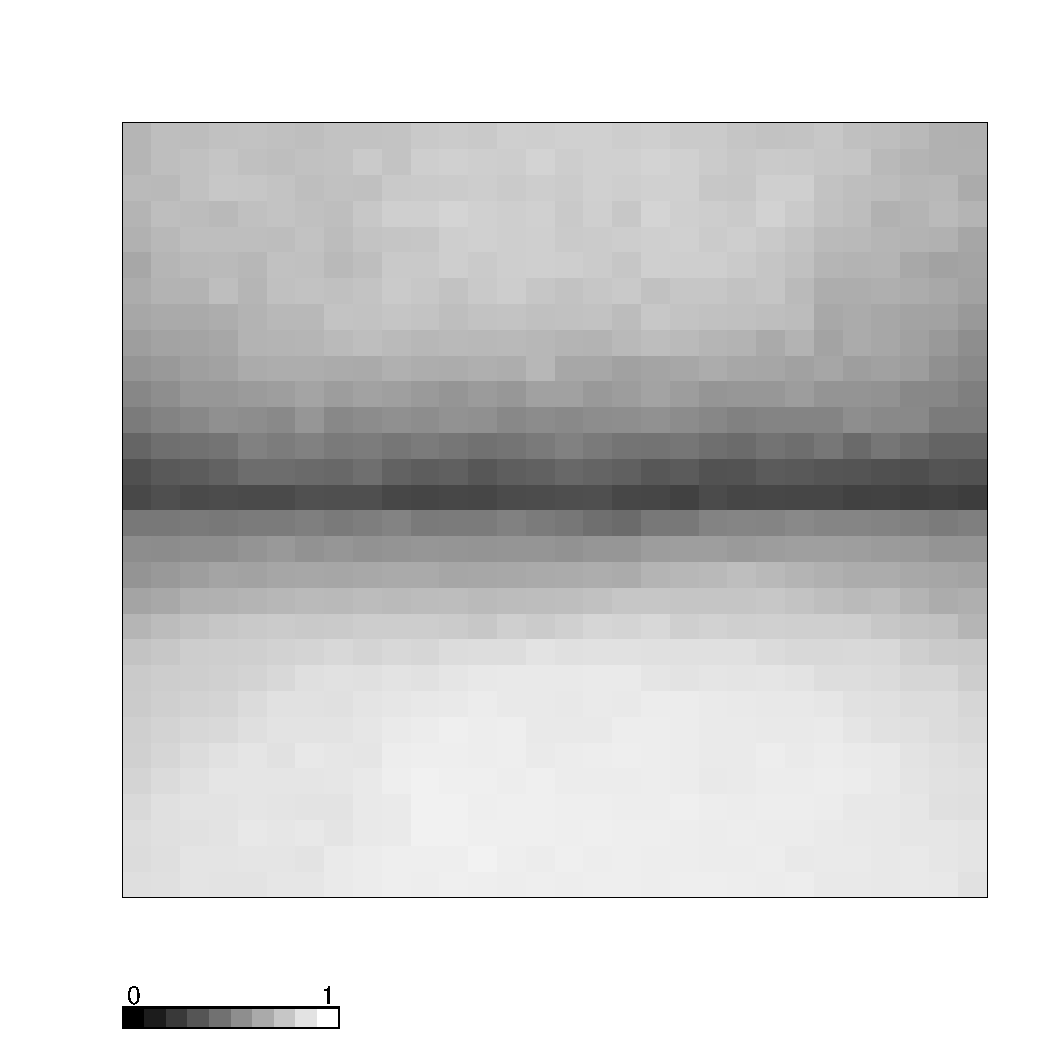
\includegraphics[width=3.1in]{../../figures/simulation/X1.coverage.pdf}
						\label{figX1:subfig1}
					}
					\subfigure[Selection frequency for $X_1$]{
						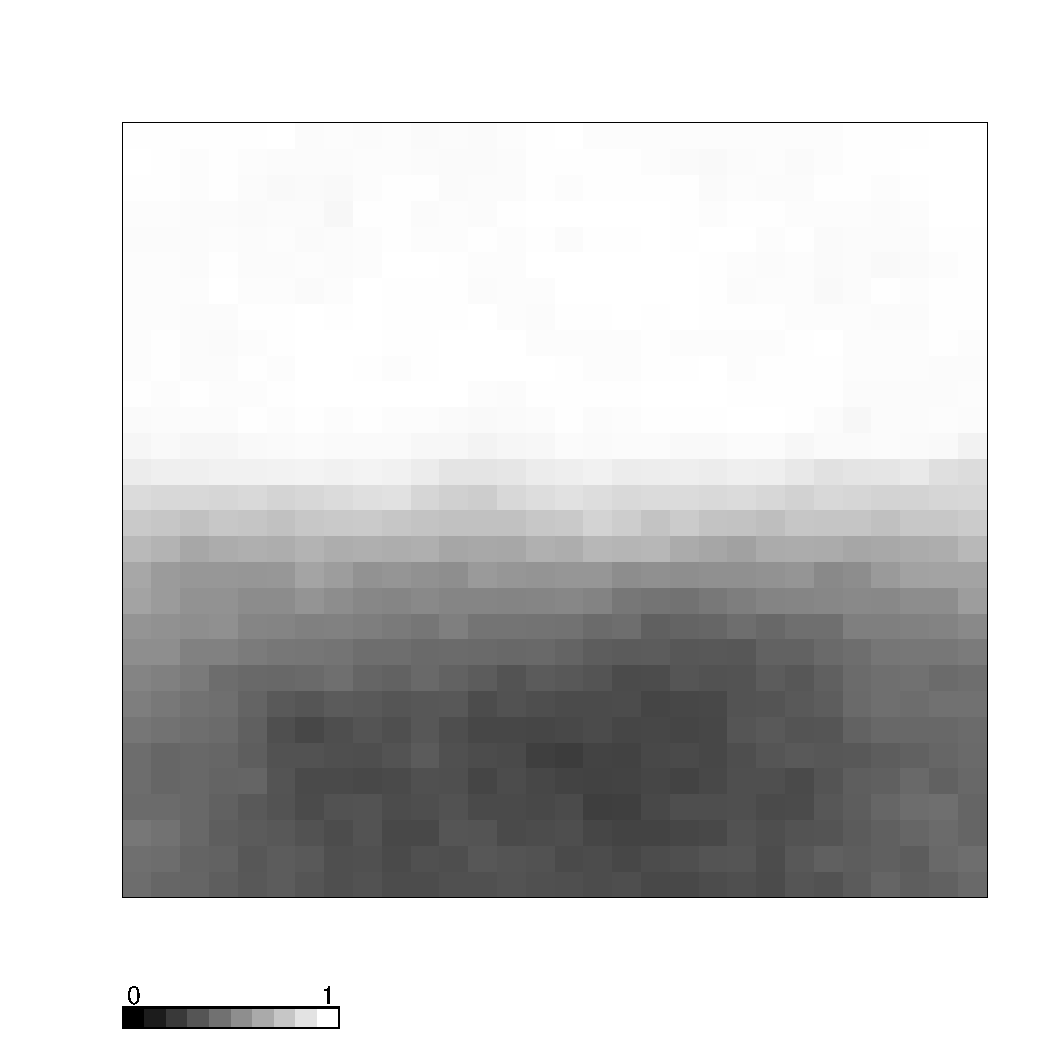
\includegraphics[width=3.1in]{../../figures/simulation/X1.selection.pdf}
						\label{figX1:subfig2}
					}
					\caption{Confidence interval coverage and selection frequency for $X_1$.\label{figX1}}
				\end{center}
			\end{figure}
					
					
			\begin{figure}
				\begin{center}
					\subfigure[Coverage of 95\% CI for $X_2$]{
						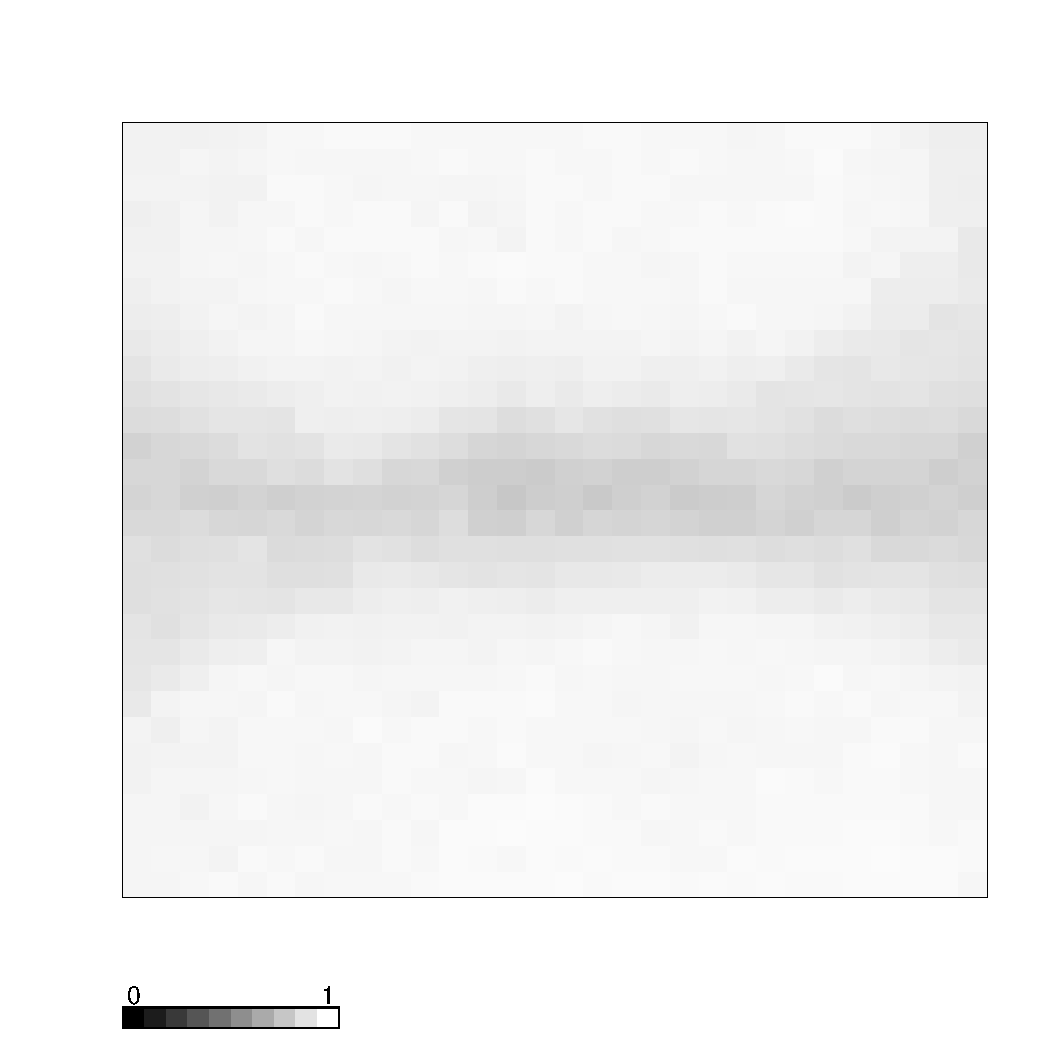
\includegraphics[width=3.1in]{../../figures/simulation/X2.coverage.pdf}
						\label{figX2:subfig1}
					}
					\subfigure[Selection frequency for $X_2$]{
						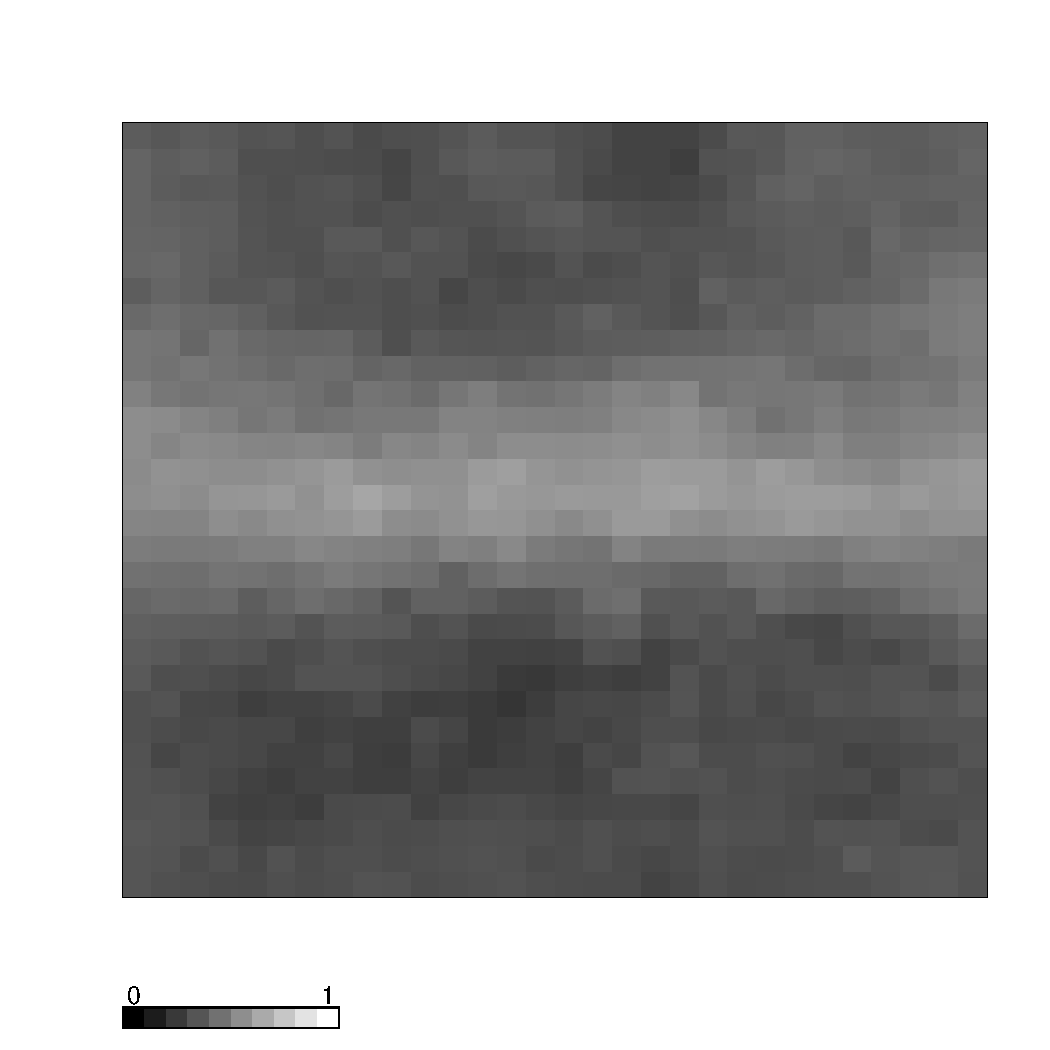
\includegraphics[width=3.1in]{../../figures/simulation/X2.selection.pdf}
						\label{figX2:subfig2}
					}									
					\caption{Confidence interval coverage and selection frequency for $X_2$.\label{figX2}}
				\end{center}
			\end{figure}
			
			
			\begin{figure}
				\begin{center}
					\subfigure[Coverage of 95\% CI for $X_3$]{
						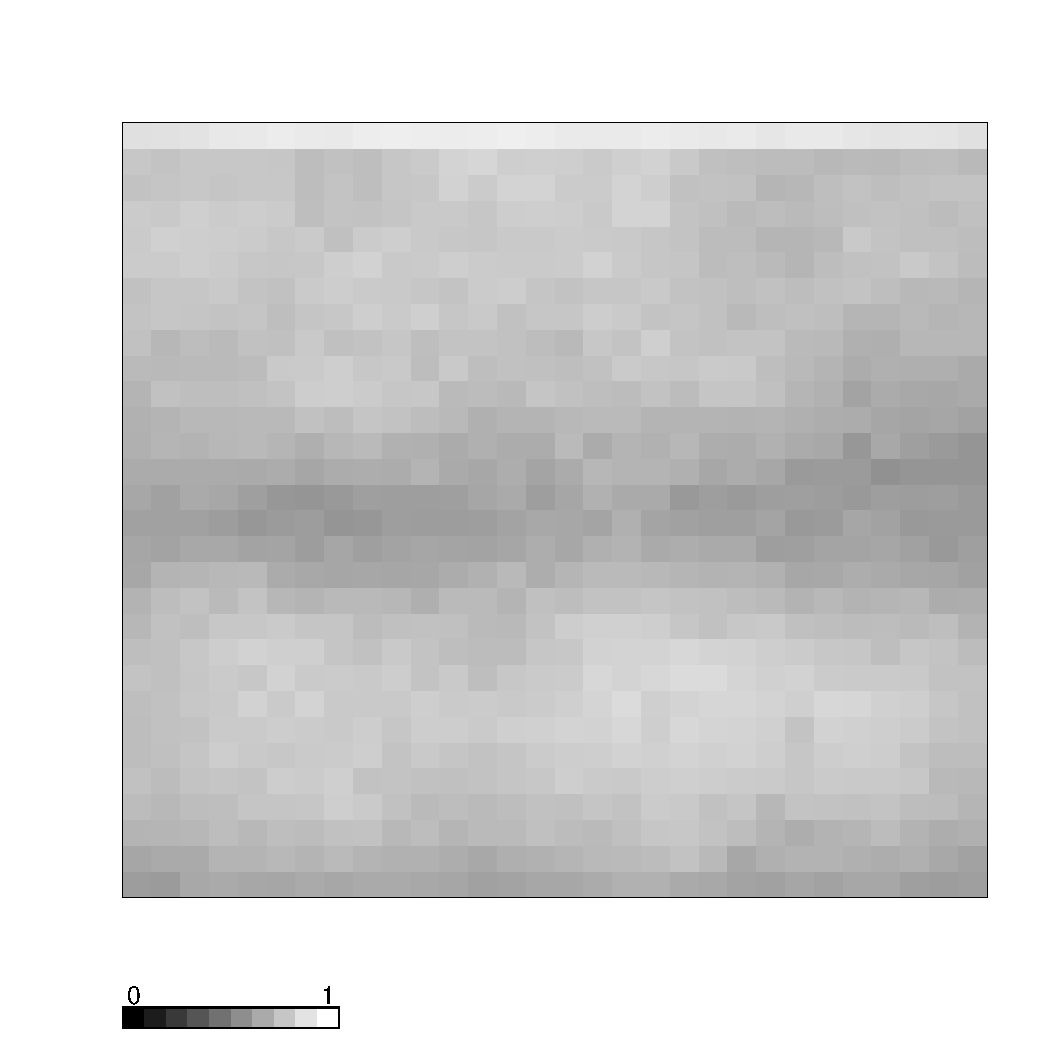
\includegraphics[width=3.1in]{../../figures/simulation/X3.coverage.pdf}
						\label{figX3:subfig1}
					}
					\subfigure[Selection frequency for $X_3$]{
						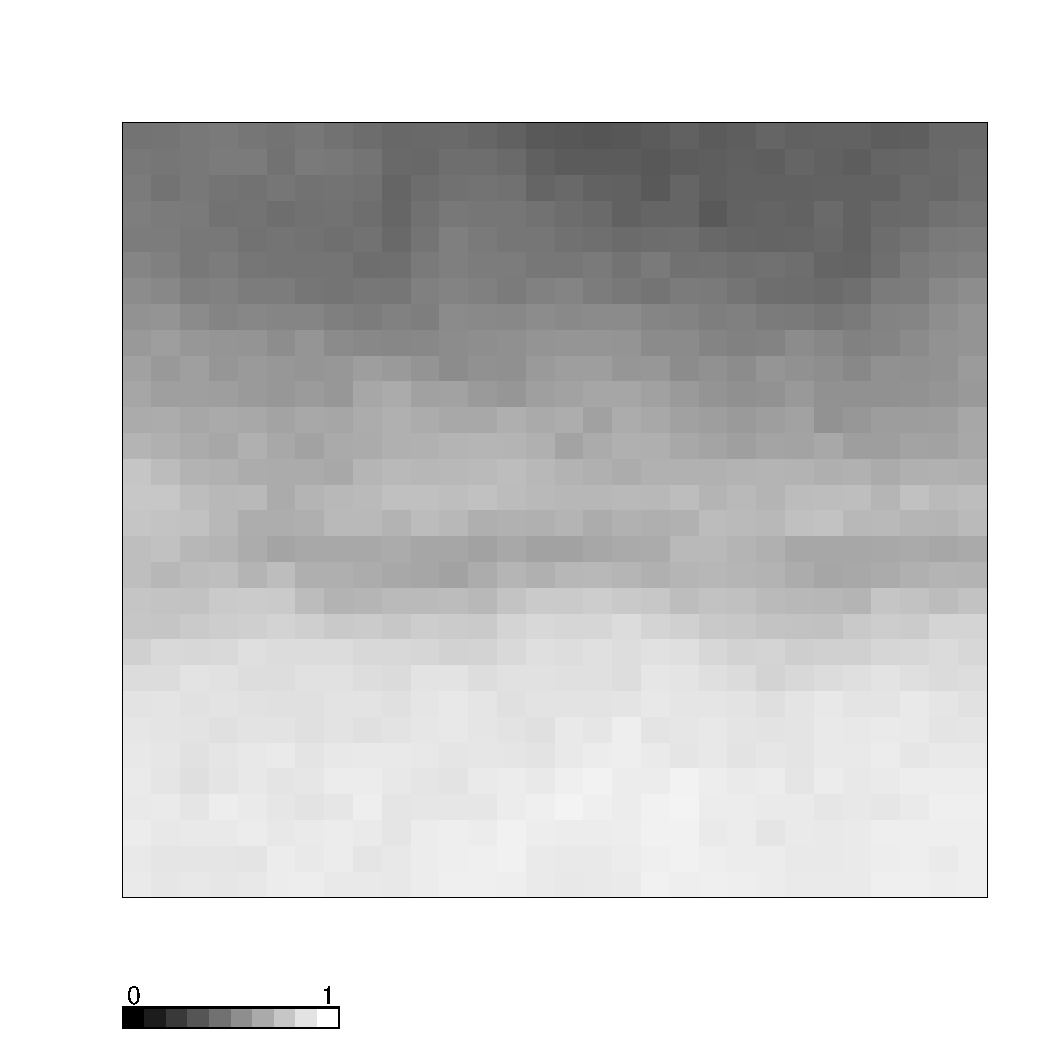
\includegraphics[width=3.1in]{../../figures/simulation/X3.selection.pdf}
						\label{figX3:subfig2}
					}									
					\caption{Confidence interval coverage and selection frequency for $X_3$.\label{figX3}}
				\end{center}
			\end{figure}
			
			
			\begin{figure}
				\begin{center}
					\subfigure[Coverage of 95\% CI for $X_4$]{
						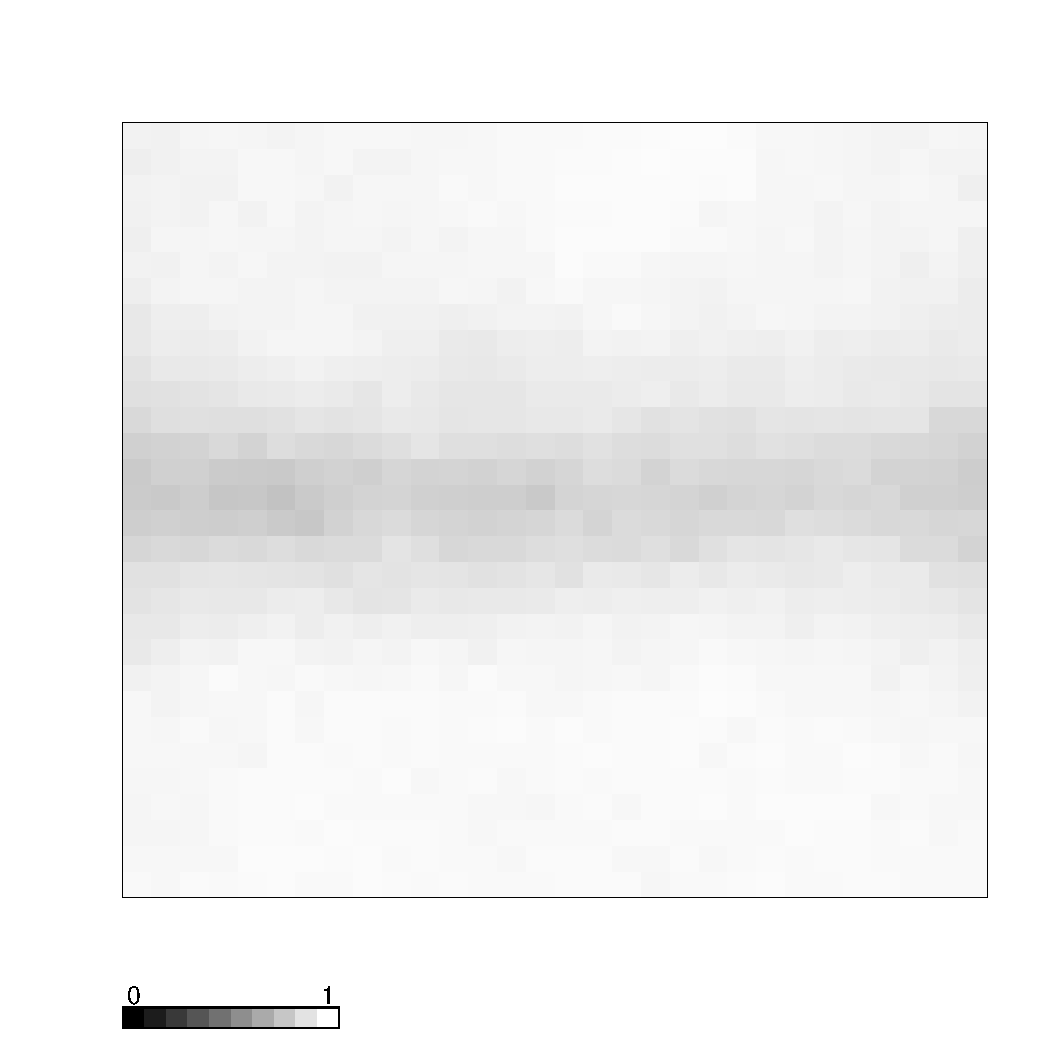
\includegraphics[width=3.1in]{../../figures/simulation/X4.coverage.pdf}
						\label{figX4:subfig1}
					}
					\subfigure[Selection frequency for $X_4$]{
						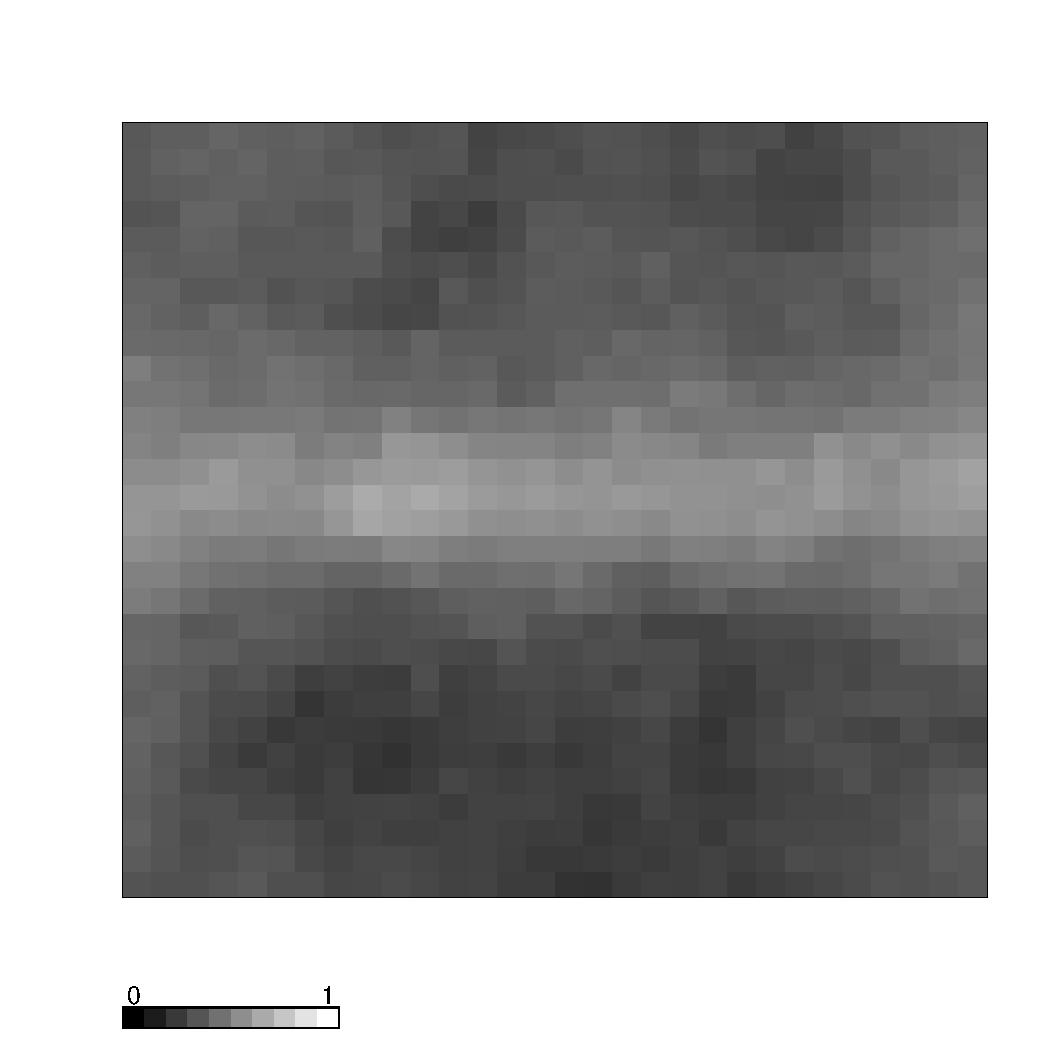
\includegraphics[width=3.1in]{../../figures/simulation/X4.selection.pdf}
						\label{figX4:subfig2}
					}									
					\caption{Confidence interval coverage and selection frequency for $X_4$.\label{figX4}}
				\end{center}
			\end{figure}
			
			
			\begin{figure}
				\begin{center}
					\subfigure[Coverage of 95\% CI for $X_5$]{
						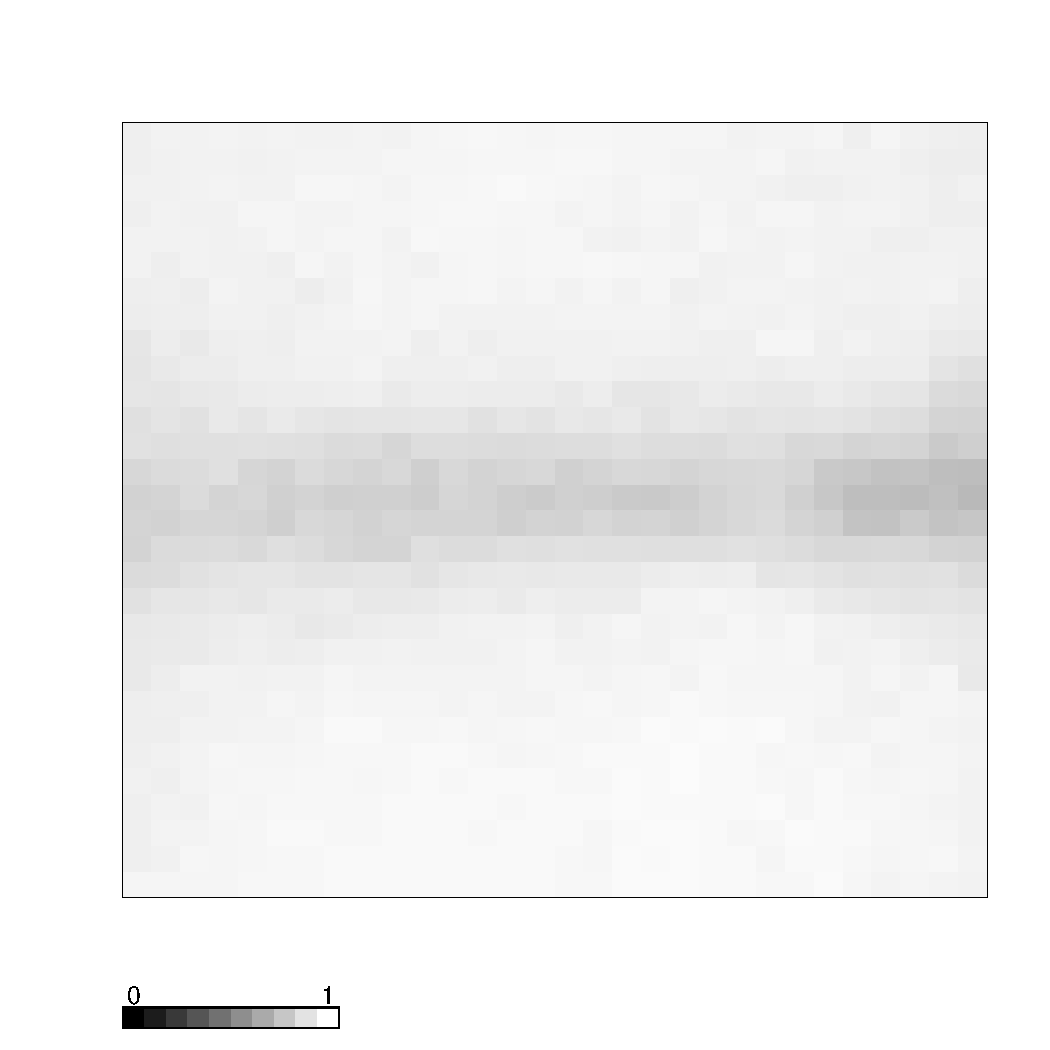
\includegraphics[width=3.1in]{../../figures/simulation/X5.coverage.pdf}
						\label{figX5:subfig1}
					}
					\subfigure[Selection frequency for $X_5$]{
						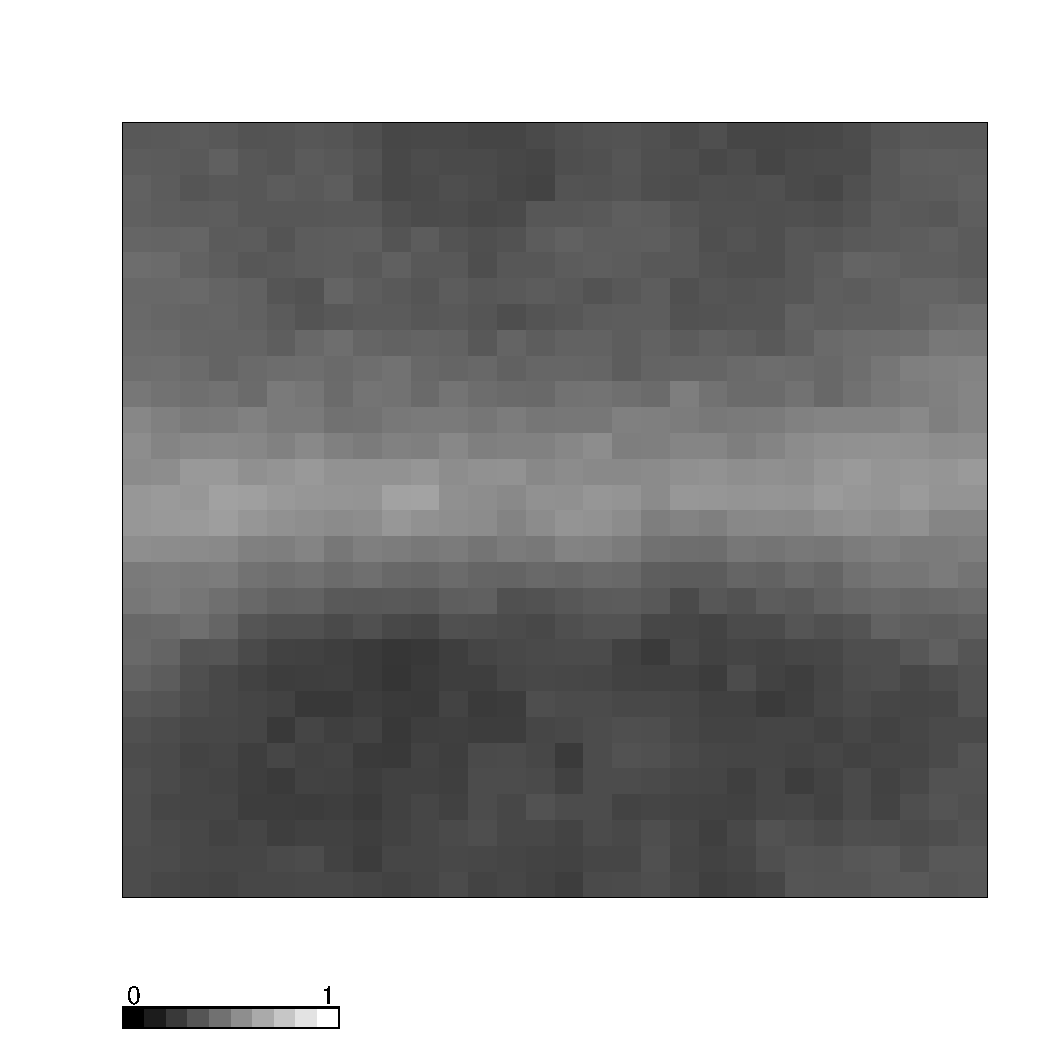
\includegraphics[width=3.1in]{../../figures/simulation/X5.selection.pdf}
						\label{figX5:subfig2}
					}									
					\caption{Confidence interval coverage and selection frequency for $X_5$.\label{figX5}}
				\end{center}
			\end{figure}
			
			
			\begin{figure}
				\begin{center}
					\subfigure[Coverage of 95\% CI for $Z$]{
						
\includegraphics[width=3.1in]{../../figures/simulation/Z.coverage.pdf}
						\label{figZ:subfig1}
					}
					\subfigure[Selection frequency for $Z$]{
						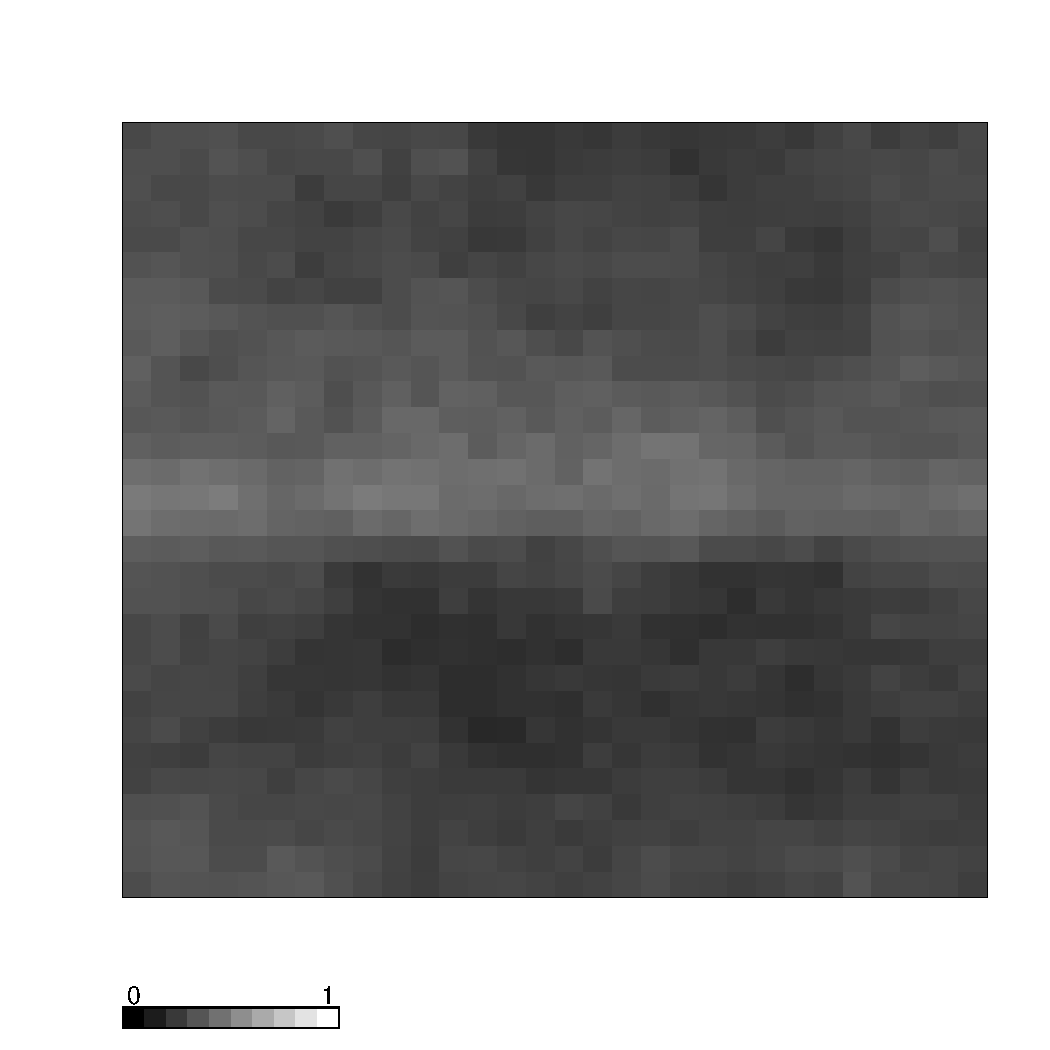
\includegraphics[width=3.1in]{../../figures/simulation/Z.selection.pdf}
						\label{figZ:subfig2}
					}									
					\caption{Confidence interval coverage and selection frequency for $Z$.\label{figZ}}
				\end{center}
			\end{figure}
			
			
			\begin{figure}
				\begin{center}
					\subfigure[Coverage of 95\% CI for intercept]{
						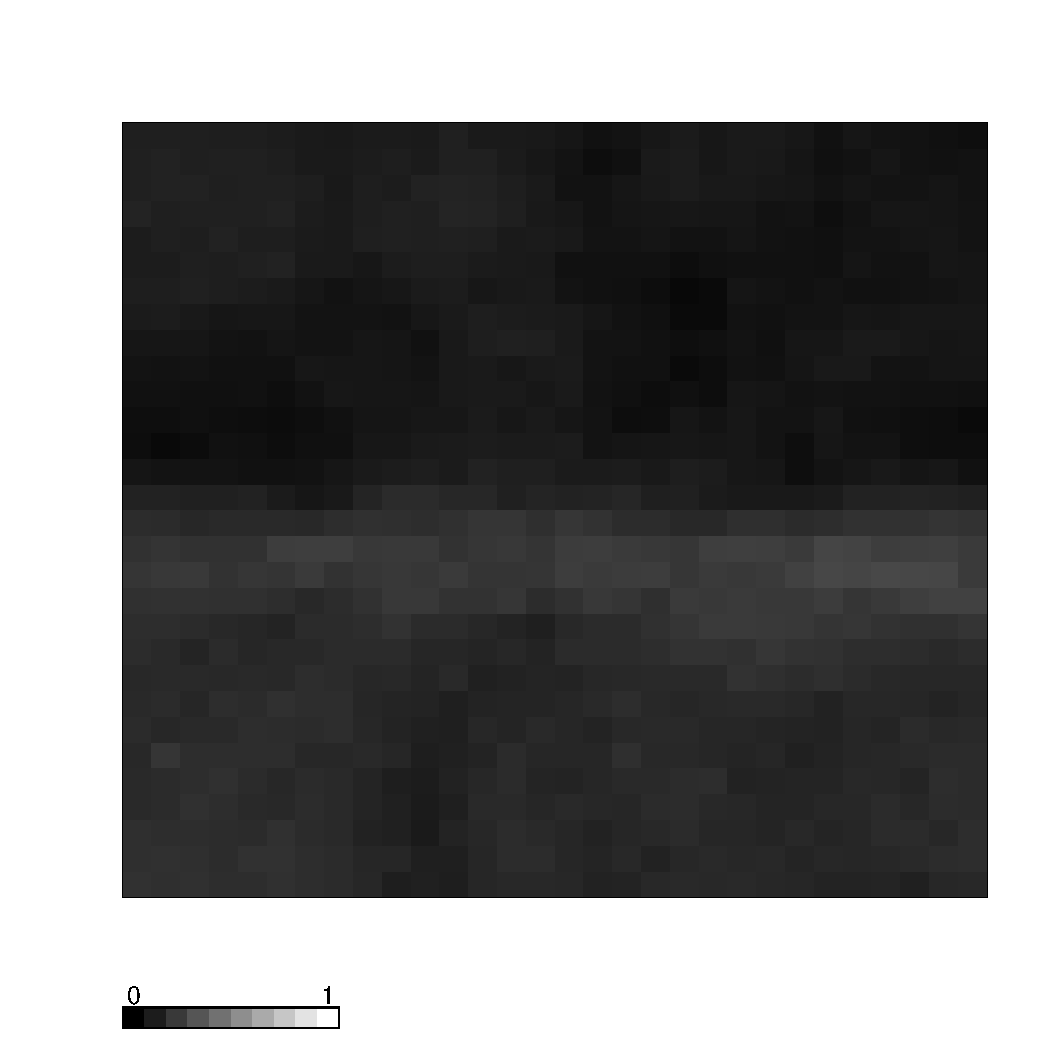
\includegraphics[width=3.1in]{../../figures/simulation/Intercept.coverage.pdf}
						\label{figIntercept:subfig1}
					}
					\subfigure[Selection frequency for intercept]{
						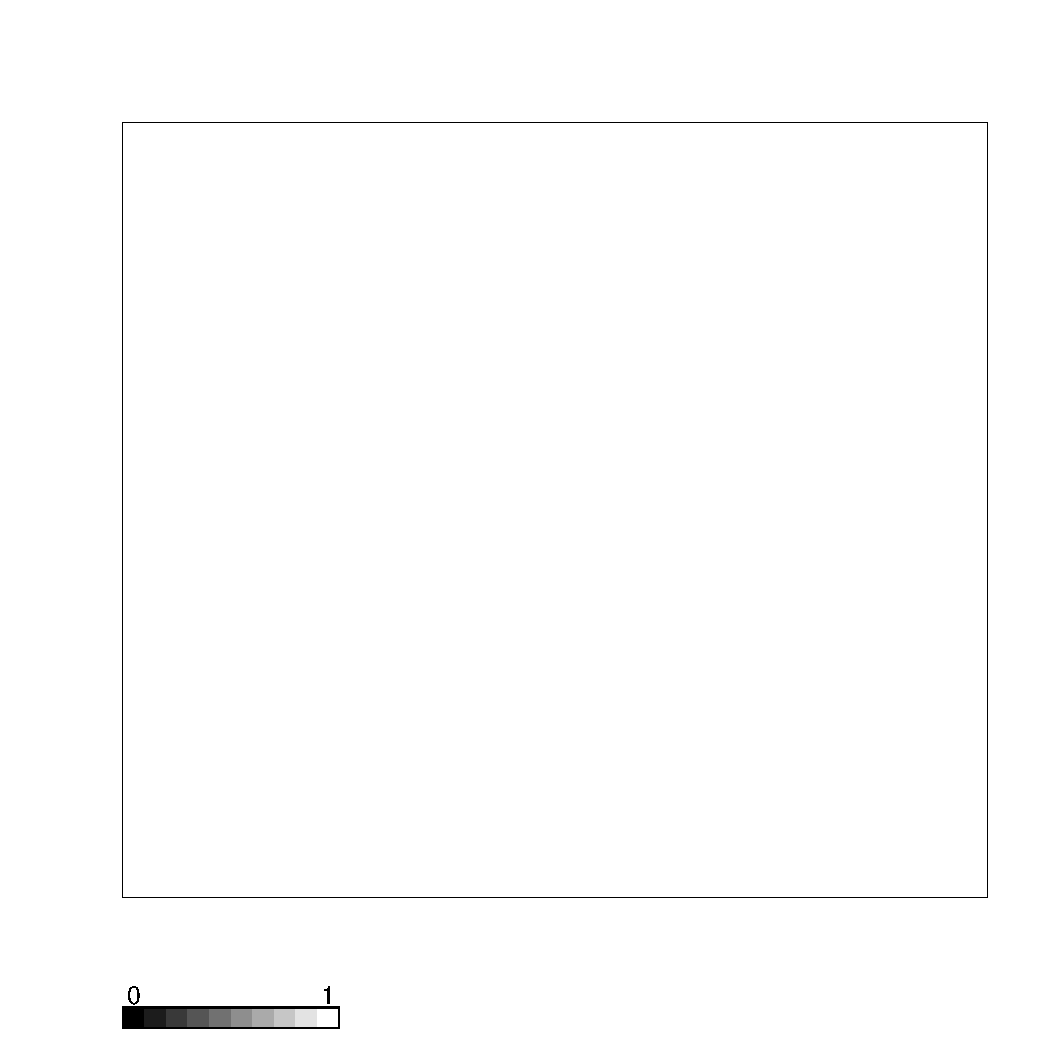
\includegraphics[width=3.1in]{../../figures/simulation/Intercept.selection.pdf}
						\label{figIntercept:subfig2}
					}									
					\caption{Confidence interval coverage and selection frequency for intercept.\label{figIntercept}}
				\end{center}
			\end{figure}
			
			\end{comment}
			
			
			
		%\subsection{Poverty data}
		%	\begin{figure}
		%		\begin{center}
		%			\includegraphics[width=5in]{../../figures/poverty/pag.estimate.pdf}
		%			\caption{Estimated coefficient surface for pag.\label{fig:pag}}
		%		\end{center}
		%	\end{figure}
		%			
		%			
		%	\begin{figure}
		%		\begin{center}
		%			\includegraphics[width=5in]{../../figures/poverty/pex.estimate.pdf}
		%			\caption{Estimated coefficient surface for pex.\label{fig:pex}}
		%		\end{center}
		%	\end{figure}
		%				
		%	
		%	\begin{figure}
		%		\begin{center}
		%			\includegraphics[width=5in]{../../figures/poverty/pman.estimate.pdf}
		%			\caption{Estimated coefficient surface for pman.\label{fig:pman}}
		%		\end{center}
		%	\end{figure}
		%				
		%	
		%	\begin{figure}
		%		\begin{center}
		%			\includegraphics[width=5in]{../../figures/poverty/pserve.estimate.pdf}
		%			\caption{Estimated coefficient surface for pserve.\label{fig:pserve}}
		%		\end{center}
		%	\end{figure}
		%				
		%	
		%	\begin{figure}
		%		\begin{center}
		%			\includegraphics[width=5in]{../../figures/poverty/pfire.estimate.pdf}
		%			\caption{Estimated coefficient surface for pfire.\label{fig:pfire}}
		%		\end{center}
		%	\end{figure}
		%				
		%	
		%	\begin{figure}
		%		\begin{center}
		%			\includegraphics[width=5in]{../../figures/poverty/potprof.estimate.pdf}
		%			\caption{Estimated coefficient surface for potprof.\label{fig:potprof}}
		%		\end{center}
		%	\end{figure}
		%	
		%	
		%	
		%	\begin{figure}
		%		\begin{center}
		%			\includegraphics[width=5in]{../../figures/poverty/pwh.estimate.pdf}
		%			\caption{Estimated coefficient surface for pwh.\label{fig:pwh}}
		%		\end{center}
		%	\end{figure}
		%				
		%	
		%	\begin{figure}
		%		\begin{center}
		%			\includegraphics[width=5in]{../../figures/poverty/pblk.estimate.pdf}
		%			\caption{Estimated coefficient surface for pblk.\label{fig:pblk}}
		%		\end{center}
		%	\end{figure}
		%				
		%	
		%	\begin{figure}
		%		\begin{center}
		%			\includegraphics[width=5in]{../../figures/poverty/phisp.estimate.pdf}
		%			\caption{Estimated coefficient surface for phisp.\label{fig:phisp}}
		%		\end{center}
		%	\end{figure}
		%				
		%	
		%	\begin{figure}
		%		\begin{center}
		%			\includegraphics[width=5in]{../../figures/poverty/metro.estimate.pdf}
		%			\caption{Estimated coefficient surface for metro.\label{fig:metro}}
		%		\end{center}
		%	\end{figure}
			


			
\section{References}
\bibliographystyle{chicago}
\bibliography{../../references/gwr}

\end{document}  